\chapter{Spectral Method}
\label{chap:spectral-method}

\section{Definitions}
\input{chapters/out/Spectral Method.md.tex}

\begin{definition}{Ansatz}{}\input{chapters/out/Ansatz.md.tex}\end{definition}
\begin{definition}{Bound on the Error}{}\input{chapters/out/Bound on the Error.md.tex}\end{definition}
\begin{definition}{Chebyshev Polynomials}{}\input{chapters/out/Chebyshev Polynomials.md.tex}\end{definition}
\begin{definition}{Clarabel}{}\input{chapters/out/Clarabel.md.tex}\end{definition}
\begin{definition}{Derivation of In-Operator Recurrence}{}\input{chapters/out/Derivation of In-Operator Recurrence.md.tex}\end{definition}
\begin{definition}{Equilibrium Measures}{}\input{chapters/out/Equilibrium Measures.md.tex}\end{definition}
\begin{definition}{Function Space}{}\input{chapters/out/Function Space.md.tex}\end{definition}
\begin{definition}{Gaussian Hypergeometric Function}{}\input{chapters/out/Gaussian Hypergeometric Function.md.tex}\end{definition}
\begin{definition}{Gegenbauer Polynomials}{}\input{chapters/out/Gegenbauer Polynomials.md.tex}\end{definition}
\begin{definition}{Generalised Hypergeometric Series}{}\input{chapters/out/Generalised Hypergeometric Series.md.tex}\end{definition}
\begin{definition}{Implementation and Results}{}\input{chapters/out/Implementation and Results.md.tex}\end{definition}
\begin{definition}{Integration Routine}{}\input{chapters/out/Integration Routine.md.tex}\end{definition}
\begin{definition}{Jacobi Matrix}{}\input{chapters/out/Jacobi Matrix.md.tex}\end{definition}
\begin{definition}{Jacobi Polynomials}{}\input{chapters/out/Jacobi Polynomials.md.tex}\end{definition}
\begin{definition}{Leapfrog Integration}{}\input{chapters/out/Leapfrog Integration.md.tex}\end{definition}
\begin{definition}{Operator}{}\input{chapters/out/Operator.md.tex}\end{definition}
\begin{definition}{Orthogonal Polynomials}{}\input{chapters/out/Orthogonal Polynomials.md.tex}\end{definition}
\begin{definition}{Outer Optimisation Routine}{}\input{chapters/out/Outer Optimisation Routine.md.tex}\end{definition}
\begin{definition}{Rising Factorial}{}\input{chapters/out/Rising Factorial.md.tex}\end{definition}
\begin{definition}{Rust Conference}{}\input{chapters/out/Rust Conference.md.tex}\end{definition}
\begin{definition}{Spectral Convergence}{}\input{chapters/out/Spectral Convergence.md.tex}\end{definition}
\begin{definition}{Theorem 2.16}{}\input{chapters/out/Theorem 2.16.md.tex}\end{definition}
\begin{definition}{Three-Term Recurrence Relationship}{}\input{chapters/out/Three-Term Recurrence Relationship.md.tex}\end{definition}

\begin{theorem}{Integration Theorem that needs a name}{theorem216}
  On the $d$-dimensional unit ball $B_1$ the power law potential, with power $\alpha \in(-d,2+2m-d)$, $m\in\mathbb{N}_0$ and $\beta>-d$, of the $n$-th weighted radial Jacobi polynomial $$(1-|y|^2)^{m-\frac{\alpha+d}{2}}P_n^{(m-\frac{\alpha+d}{2},\frac{d-2}{2})}(2|y|^2-1)$$ reduces to a Gaussian hypergeometric function as follows:
  \begin{align*}
    \int_{B_1} & |x-y|^\beta (1-|y|^2)^{m-\frac{\alpha+d}{2}} P_n^{(m-\frac{\alpha+d}{2},\frac{d-2}{2})}(2|y|^2-1) \mathrm{d}y                                                                                                                                                                                                                                                                                               \\
               & = \tfrac{\pi ^{d/2} \Gamma \left(1+\frac{\beta}{2}\right) \Gamma \left(\frac{\beta+d}{2}\right) \Gamma \left(m+n-\frac{\alpha+d}{2}+1\right)}{\Gamma \left(\frac{d}{2}\right) \Gamma (n+1) \Gamma \left(\frac{\beta}{2}-n+1\right) \Gamma \left(\frac{\beta-\alpha}{2}+m+n+1\right)}{}_2F_1\left(\begin{matrix}n-\frac{\beta}{2}, \quad -m-n+\frac{\alpha-\beta}{2} \\\frac{d}{2}\end{matrix};|x|^2\right).
  \end{align*}
\end{theorem}

\section{Derivation of Operator}
Based on the {[}{[}Three-Term Recurrence Relationship{]}{]}.

One can even determine an explicit relationship between the coefficients
in the Jacobi expansion by considering the {[}{[}Jacobi Matrix{]}{]}.

Considering the operator $\hat{Q}^\beta[\rho]$ as in \Cref{thm:theorem216}, from the [[Ansatz]] $\rho(x)$ we have
$$\hat{Q}^{\beta}(x) = \sum_{k=1}^{N} \rho_{k} \int \norm{x-y}^{\beta}(1-\norm{y}^2)^{a}P_{k}^{(a, b)}(2\norm{y}^{2}- 1) \,\ddy$$


\begin{figure}[H]
  \centering
  \label{fig:attractive-repulsive}
  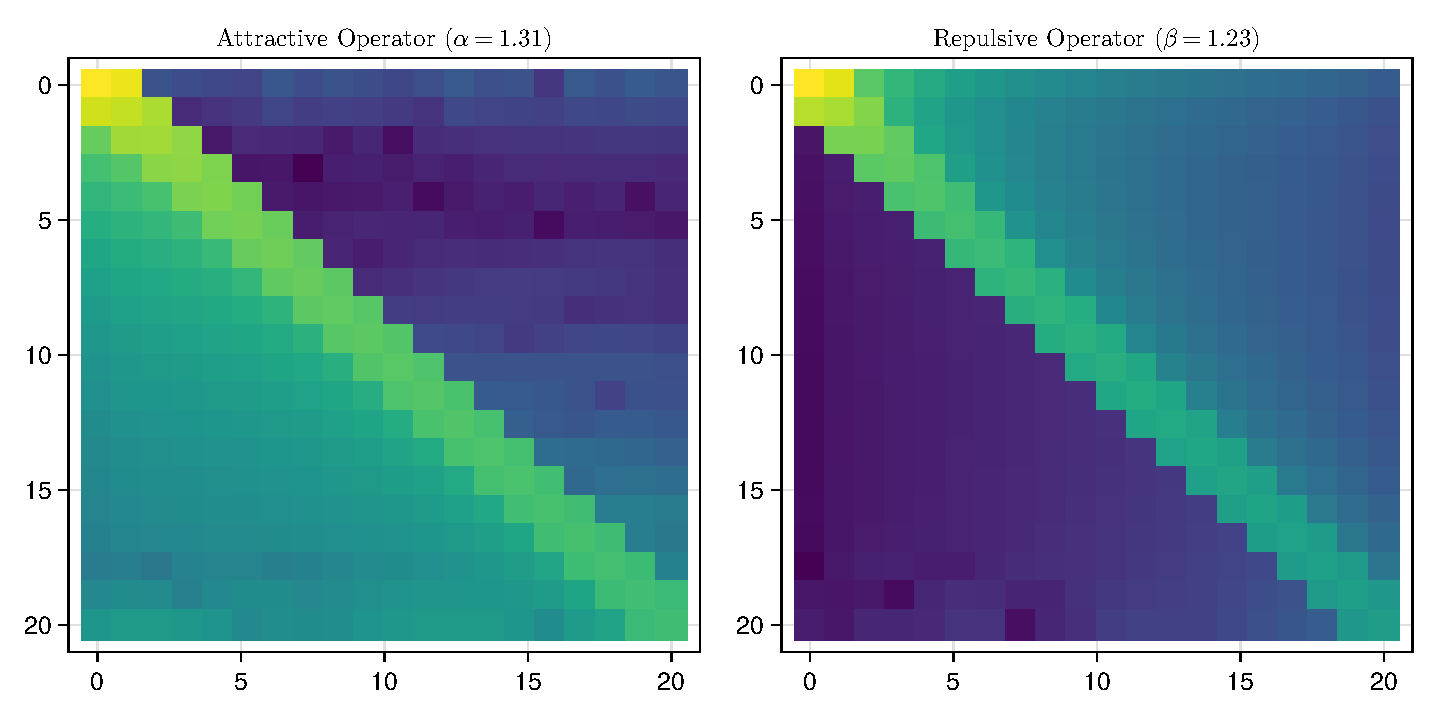
\includegraphics[width=\linewidth]{../figures/results/attractive-repulsive-operator.pdf}
  \caption{The attractive and repulsive operators}
\end{figure}
